% Chapter 4

\chapter{Analysis and interpretation} % Main chapter title

\label{Chapter4} % For referencing the chapter elsewhere, use \ref{Chapter1} 

%----------------------------------------------------------------------------------------

\section{Summary of data collected}
In order to answer the research questions (2.1), three cases of forks with different outcomes were selected. Forking reasons and outcomes are characterized here using the terminology introduced by \citet{Robles2012a}.

\subsubsection{MySQL server / MariaDB server}
The open source database server MySQL was purchased by Sun Inc. in 2008, resulting in the departure of the original chief engineer (on good terms) to form his own company, MariaDB \citep{Widenius2009}. Subsequently, Sun was acquired by Oracle. Oracle’s attempt to highjack the project \citep{Nyman2013a} led to a full-fledged fork in 2012 \citep{Widenius2012}.

\begin{description}
  \dt{Repositories}
  \dd{
    MySQL \\ https://github.com/mysql/mysql-server.git \\
    MariaDB \\ https://github.com/MariaDB/server.git
  }
  
  \dt{Reasons for the fork}
  \dd{Technical, more community-driven development, legal issues.}

  \dt{Outcome}
  \dd{Competition, successful branching, with differentiation.}
\end{description}

\subsubsection{Linux kernel / Android kernel}
In 2005, Google Inc. bought Android, then a start-up developing a Linux-based operating system for cellular phones, in order to expand its search service to the mobile market \citep{Elgin2005}. The Linux community and Google have been cooperating on the core system, while Google continues to develop device-specific extensions to the core under a shared open source licensing regime \citep{Vaughan-Nichols2011}.

\begin{description}
  \dt{Repositories}
  \dd{
    Linux \\ git://git.kernel.org/pub/scm/linux/kernel/git/torvalds/linux.git \\
    Android \\
    https://android.googlesource.com/kernel/common \\
    https://android.googlesource.com/kernel/x86\textunderscore64
  }
  
  \dt{Reasons for the fork}
  \dd{Commercial strategy, technical.}
  
  \dt{Outcome}
  \dd{Cooperation, successful branching, with differentiation.}
\end{description}

\subsubsection{Apache OpenOffice / LibreOffice}
Development of the OpenOffice suite of office applications began in 2000, in a company owned by Sun Microsystems; following the acquisition of Sun by Oracle, OpenOffice was forked into LibreOffice by its developers in 2010; as OpenOffice lost momentum, Oracle donated the project to the Apache foundation in 2011 \citep{Gamalielsson2014b}.

\begin{description}
  \dt{Repositories}
  \dd{
    Apache OpenOffice \\ https://github.com/apache/openoffice.git \\
    LibreOffice \\ git://anongit.freedesktop.org/libreoffice
  }
  
  \dt{Reasons for the fork}
  \dd{More community-driven development, discontinuation of the original project.}

  \dt{Outcome}
  \dd{Discontinuation of the original, successful continuation of the fork.}
\end{description}

\subsection{Data acquisition}
In order to make the data easier to process, a database was populated with data obtained from the projects' repositories (\ref{AppendixA}). A script was written in Python to collect the data from the software repositories, and a second script to compute the metrics. The scripts were written applying test-driven-development to ensure their correctness and maintainability. Data collection was automated, so the process is repeatable.

Team members were identified by their login name, publicly available through the repositories’ logs. Login names were replaced by non-reversible unique hashes prior to being stored in a local database (in line with ethical considerations in paragraph 3.4).

The raw data as obtained from the repositories and stored in the local database is summarized in table \ref{table:ch4_rawdata}.

%-- table ----------
\begin{table}[H]
\caption{Raw data characteristics (database entry counts).}
\label{table:ch4_rawdata} 
\centering
\begin{tabu} to \linewidth{lrrrrrr}
  \toprule
  & \multicolumn{2}{c}{Fork 1} & \multicolumn{2}{c}{Fork 2} & \multicolumn{2}{c}{Fork 3} \\
  \midrule
  Project & \textbf{MySQL} & \textbf{MariaDB} & \textbf{Linux} & \textbf{Android} & \textbf{OpenOffice} & \textbf{LibreOffice} \\
  \midrule
  Releases & 51 & 57 & 32 & 31 & 8 & 85 \\
  \midrule
  Files & \num{33141} & \num{29013} & \num{85421} & \num{77670} & \num{67964} & \num{162883} \\
  \midrule
  File versions & \num{871041} & \num{1045377} & \num{1427758} & \num{1376099} & \num{497036} & \num{5685337} \\
  \midrule
  Contributors & \num{1230} & \num{1320} & \num{16081} & \num{16325} & 42 & \num{1219} \\
  \midrule
  Edits and \\commits \\combined & \num{8236} & \num{8725} & \num{57103} & \num{37654} & 164 & \num{6999} \\
  \bottomrule
\end{tabu}
\end{table}


\subsection{Exporting and recoding the data for analysis}
The measurements obtained from the data were exported in a format suitable for analysis: a spreadsheet where columns represent releases and rows represent measured characteristics.

\begin{itemize}
\item{For code characteristics, one column for each release and 2 rows for each file: "presence/absence" and "checksum".}
\item{For team characteristics, one column for each release and 3 rows for each contributor: "presence/absence" in team, "edits count" and "commits count".
A Python script was written to export the data. The script handles re-encoding and cleaning-up the data, discussed below.}
\end{itemize}

\subsubsection{Re-encoding}
Binary characters, e.g. presence/absence of a file in a branch, were encoded as a row of Boolean values. Count characters were encoded as integers. Measurement characters, e.g. checksums of files, were recoded into classes: if a file is the same for all branches, there was only one class, if a file changes in all branches, there were as many classes as branches and so on (see table 3.1 for an overview of the data types used).

\subsubsection{Cleaning-up}
The data had to be cleaned-up before processing: only rows which are complete could be used for calculating the distance matrix, e.g. if a file is missing in a release, its corresponding “checksum” row had to be discarded. Cleaned-up data represents between 53 and 64 \% of the raw data, depending on the fork (table \ref{ch4_cleanup}).

%-- table ----------
\begin{table}[H]
\caption{Measurement characteristics (spreadsheet row counts), after clean-up.}
\label{table:ch4_cleanup} 
\centering
\begin{tabu} to \linewidth{P{4cm}rrr}
  \toprule
  Characteristic & MySQL / MariaDB & Linux / Android & OpenOffice / LibreOffice \\
  \midrule
  File version presence / absence & \num{51209} & \num{87706} & \num{171695} \\
  \midrule
  File version checksum & \num{621} & \num{6705} & \num{23905} \\
  \midrule
  Contributor presence / absence & \num{1505} & \num{16325} & \num{1232} \\
  \midrule
  Edit count per contributor & \num{1505} & \num{16325} & \num{1232} \\
  \midrule
  Commit count per contributor & \num{1505} & \num{16325} & \num{1232} \\
  \midrule
  Total number of columns (branches) & 107 & 63 & 93 \\
  \midrule
  Total number of rows (characteristics) & \num{56648} & \num{144299} & \num{199296} \\
  \midrule
  Percentage of raw data after clean-up & 53\% & 64\% & 57\% \\
  \bottomrule
\end{tabu}
\end{table}


\subsection{Applying phylogenetic methods}
Distance matrices were computed and phylogenetic trees were estimated for each fork case studied. The software was written using the R language for statistical computing \citep{RDevelopmentCoreTeam2008a}. The classes implemented are wrappers for the R functions provided by packages for general and biological statistics. 

The software implemented for the research is documented in the class diagram in \ref{AppendixB}.

\begin{itemize}
\item{Distance matrices were calculated using the function “gower” provided by the R-package “StatMatch” \citep{DOrazio2016}.}

\item{The UPGMA technique for computing taxonomic trees (3.1.3) was implemented using the function ”hclust” with the agglomeration method “UPGMA” provided by the R-package “Stats” \citep[p.1355]{RDevelopmentCoreTeam2008a}.}

\item{The Neighbour-Joining and Minimum Evolution techniques (3.1.3) were implemented using the functions “nj” and “fastme.bal” provided by the R-package “Ape” \citep{Paradis2004a}.}
\end{itemize}

\subsection{Cophenetic distances}
Answering the research questions involves calculating a cophenetic distance matrix for each tree. Cophenetic distances were calculated using the function “cophenetic” provided by the R-package “Stats” \citep[p.1275]{RDevelopmentCoreTeam2008a}.

%----------------------------------------------------------------------------------------

\section{Data analysis}

\subsection{Answering RQ1}
Answering RQ1 (see paragraph 2.1) requires calculating the distance between software releases and estimating if these distances correlate to forks and branches. The expected outcome is that forks will always differ more than branches, independently of the outcome of the project.

\subsubsection{Choice of statistical method for analysis}
Whether a pair of releases represents a fork or a branch is a nominal variable with two possible values (“fork” or “branch”) and the pairwise cophenetic distance between releases is a measurement variable. A suitable test for these types of variables is a one-way analysis of variance (ANOVA) with two categories \citep{McDonald2014b}. The result should be repeatable for each case described in 4.1. The R-package “Stats” provides methods for computing variance \citep[p.1211]{RDevelopmentCoreTeam2008a}.

\subsubsection{Checking assumptions for RQ1}

\definition{Assumption 1: Accuracy}{Methods for computing trees from distance matrices are assumed to produce trees that represent the distance matrix accurately.}

\noindent
The three methods chosen in 3.1.3 (UPGMA, NJ, ME) were applied, and the correlation between the distance matrix and the cophenetic matrix obtained from each tree was used as a measure of how accurately the trees represent the distance matrix \citep{Rohlf2013a}. Correlations (Pearson's Chi-squared test) were calculated for each fork (table \ref{table:ch4_rq1_corr}). The Neighbour-Joining method was found to produce the best correlation for the 3 data sets considered (correlation > 0.991086), UPGMA is second (correlation > 0.823779) and ME is the most inaccurate method (correlation > 0.512404).

%-- table ----------
\begin{table}[H]
\caption{Correlations between distance and cophenetic matrices for each fork and method.}
\label{table:ch4_rq1_corr} 
\centering
\begin{tabu} to \linewidth{P{5cm}P{3cm}P{3cm}P{2cm}}
  \toprule
  Projects (code and team measurements) & Method used to estimate the tree & Correlation between distance matrix and tree & p-value * \\
  \midrule  
  \multirow{3}{*}{MySQL / MariaDB} & UPGMA & 0.823779 & < 2.2e-16 \\
  & NJ & 0.993690 & < 2.2e-16 \\
  & ME & 0.624948 & < 2.2e-16 \\
  \midrule  
  \multirow{3}{*}{Linux / Android} & UPGMA & 0.881565 & < 2.2e-16 \\
  & NJ & 0.994087 & < 2.2e-16 \\
  & ME & 0.512404 & < 2.2e-16 \\
  \midrule  
  \multirow{3}{*}{OpenOffice / LibreOffice} & UPGMA & 0.936611 & < 2.2e-16 \\
  & NJ & 0.991086 & < 2.2e-16 \\
  & ME & 0.983237 & < 2.2e-16 \\
  \bottomrule
\end{tabu}
\end{table}
\noindent * 2.2e-16 is the smallest non zero floating point number than can be stored on the machine used.


\definition{Assumption 2: Normality}{ANOVA assumes that the data is normally distributed (fits the Gaussian “bell curve”) and that the standard deviation is the same for the data sets examined. Performing an ANOVA on data sets that are not normally distributed increases the chance of false positives \citep[p.147]{McDonald2014b}.}

\noindent
As can be seen in figure \ref{fig:rq1_distributions}, the data is not normally distributed. An accepted remedy for this situation is to transform the data to make it fit the assumption of normality better: common transformations are to apply logarithm or square root transformations to the data \citep[p.141]{McDonald2014b}. The histograms (\ref{fig:rq1_distributions}) show that the distribution of the square root of distances (in figure \ref{fig:rq1_distributions}, bottom row) better fits the normal distribution.

\begin{figure}[H]
  \centering
  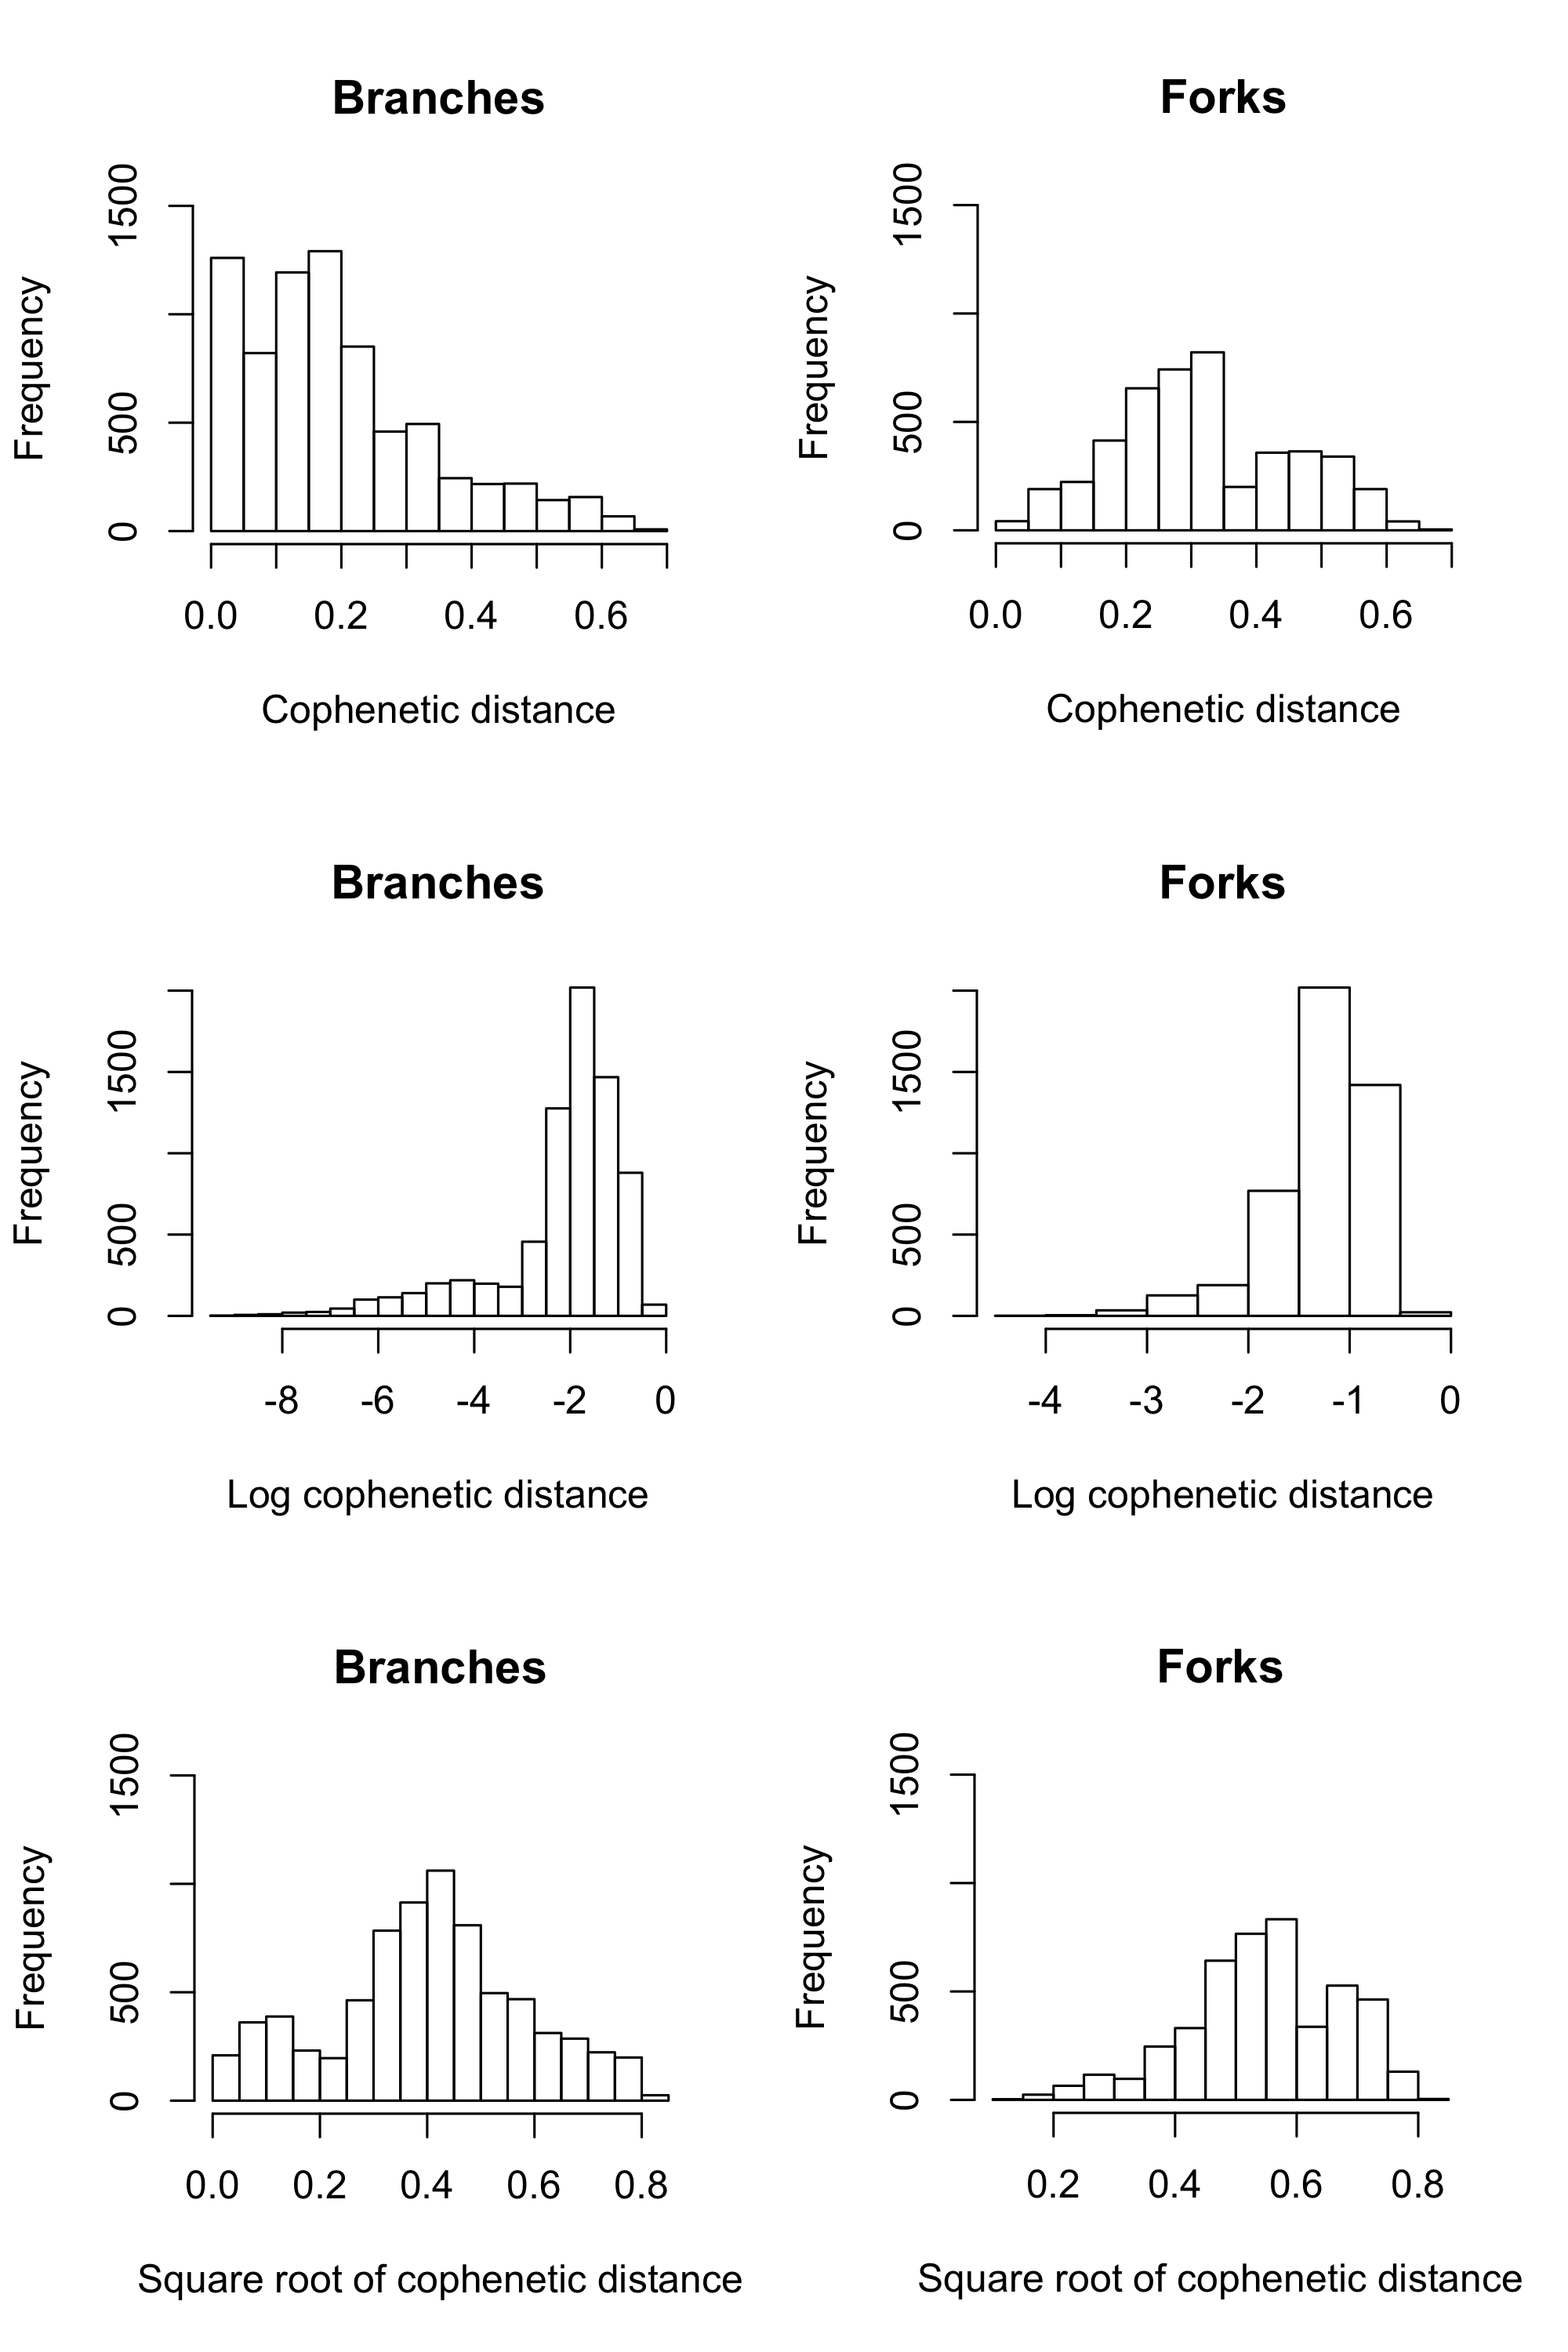
\includegraphics[width=\textwidth]{rq1_distributions.png}
  \caption{Histograms illustrating the distribution of the cophenetic distances, obtained by applying the NJ method to branches and forks of all projects considered. The top row shows untransformed distances, the middle row shows the base-10 logarithm of the distances and the bottom row the square root of the distances.}
  \label{fig:rq1_distributions}
\end{figure}

\definition{Assumption 3: Homoscedasticity}{ANOVA assumes that the standard deviation of the data is the same for the data sets considered (the data is “homoscedastic” or else it is “heteroscedastic”). Performing an ANOVA on heteroscedastic data sets increases the chance of false positives \citep[p.147]{McDonald2014b}.} Table \ref{ch4_rq1_sd.tex} shows that the cophenetic distances obtained by applying the NJ method to the square root transformed data set is homoscedastic within reason, i.e. the ratio between the standard deviation of branches and forks is relatively small (0,0020998 /  0,0018566 = 1,1309758). Therefore, performing an ANOVA on the square root transformed data should minimize the chance of false positives.

%-- table ----------
\begin{table}[H]
\caption{The standard deviations of the cophenetic distances, obtained by the NJ method for
branches and forks of all projects considered, applying the square root transformation to the data.}
\label{table:ch4_rq1_sd} 
\centering
\begin{tabu} to \linewidth{llr}
  \toprule
  Transformation applied & Release type & Standard deviation \\
  \midrule
  \multirow{2}{*}{Square root} \\
  & Branches & 0.0020998 \\
  & Forks & 0.0018566 \\
  \bottomrule
\end{tabu}
\end{table}


\subsubsection{One-way analysis of variance (ANOVA)}
The analysis involved the following steps:

\begin{enumerate}
\item{Distance matrices were computed from the data acquired for each project, using the Gower technique, as data is of various types (Boolean, integer, categorical, see table 3.1).}

\item{Trees were estimated from these distance matrices by applying the Neighbour-Joining (NJ) method, which seems to represent the distance matrix in an accurate way (as discussed under “checking assumptions for RQ1”).}
  
\item{A cophenetic distance matrix was obtained from each tree (the measurement variable).}
  
\item{Cophenetic distances were aggregated into “branches” and “forks” (the nominal variable).}

\item{One-way ANOVA was performed on the square-root of the cophenetic distances.}
\end{enumerate}

The analysis of the square root transformed data with one-way ANOVA (table \ref{table:ch4_rq1_anova}) show that the nominal variable “release type” (i.e. “branches” or “forks”) has significant influence on the cophenetic distance between releases (p < 2e-16). Therefore the null hypothesis can be rejected.

%-- table ----------
\begin{table}[H]
\caption{One-way ANOVA.}
\label{table:ch4_rq1_anova} 
\centering
\begin{tabu} to \linewidth{P{2cm}P{2cm}P{2cm}P{2cm}P{2cm}P{2cm}}
  \toprule
  Nominal variable & Degrees of freedom & Sum squares & Mean squares & F value & Pr(>F) \\
  Release type("Branches" or "Forks") & 1 & 42.62 & 42.62 & 2113 & < 2e-16 \\
  \bottomrule
\end{tabu}
\end{table}


This result is visualised in the plot in figure \ref{fig:rq1_all}: The mean cophenetic distance between releases on different forks is larger than the mean distance between releases on different branches, using data from the three projects considered.

\begin{figure}[H]
  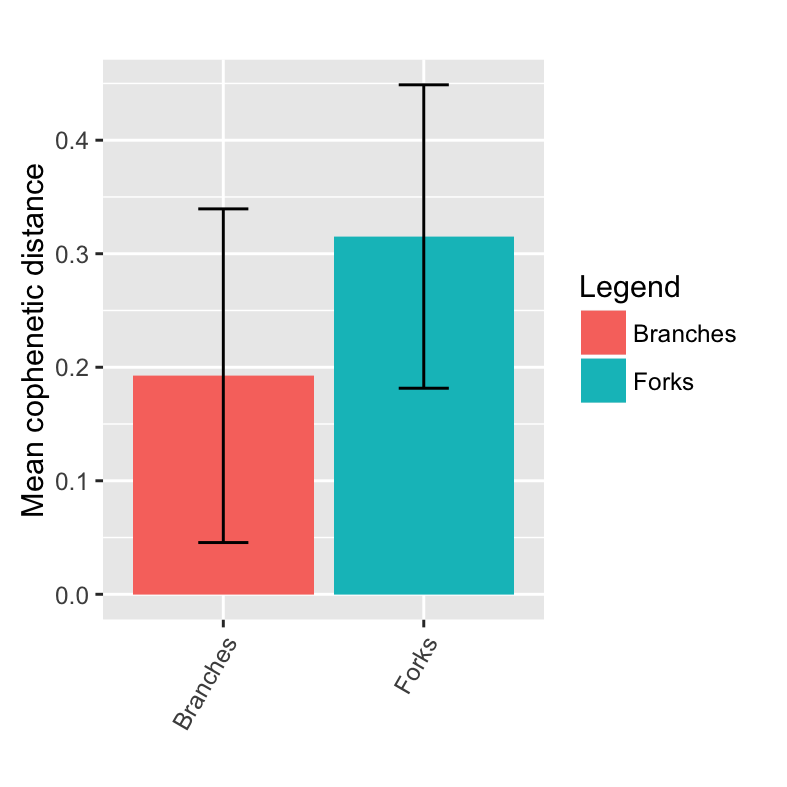
\includegraphics[width=\textwidth]{RQ1_all.png}
  \caption{Plot of the mean cophenetic distances between releases and their standard deviation for all fork cases combined.}
  \label{fig:rq1_all}
\end{figure}

\subsection{Answering RQ2}
Answering RQ2 (see paragraph 2.1) requires examining the phylogenetic trees of forks with different outcomes (competition, cooperation, discontinuation of a branch) and seeking a correlation between the outcome of the fork and the topology of the tree.

The proposed method for answering this question is to use the same approach as in RQ1, but applying it to the two data sets obtained from code measurements and team measurements, thus estimating a “code-base tree” and a “team tree” for each fork. As explained in paragraph 3.2.2, the rationale for this approach is that two distinct but cooperating teams are expected to produce a code base with many similarities, while two competing teams will produce clearly distinct code bases. Therefore answering RQ2 required treating organizational and code measurements separately. Furthermore, as different organizations and code bases were compared, measurements representing the pairwise differences between releases within the same organization, i.e. “branches”, were discarded, and only “fork” measurements were analysed.

\subsubsection{Choice of statistical method for analysis}
The outcome of a fork is a nominal variable with three categories (“competition”, “cooperation”, “discontinuation”), the data-set used to construct the tree is a second nominal variable with two categories (“code” and “team”) and the cophenetic distance between releases on different forks is a measurement variable. The null hypothesis for RQ2 is that the mean cophenetic distance is not significantly different for the “outcome” categories considered. Rejecting the null hypothesis would provide evidence that the outcome of a fork can be predicted. A suitable test for this case is a two-way ANOVA \citep{McDonald2014b}, where the measurement variable is the cophenetic distance between releases on different forks, and the two nominal variables are the outcome and the data-set used.

\subsubsection{Checking assumptions for RQ2}
The assumptions of accuracy, normality and homoscedasticity apply to a two-way ANOVA as they do to a one-way ANOVA \citep[p.176]{McDonald2014b} but have to be checked against code measurements and team measurements to answer RQ2.

\definition{Assumption 1: Accuracy}{}

\noindent
As for RQ1, the three methods chosen in 3.1.3 (UPGMA, NJ, ME) were applied, and the correlation between the distance matrix and the cophenetic matrix obtained from each tree was used as a measure of how accurately the trees represent the distance matrix \citep{Rohlf2013a}. Correlations were calculated for each data set and fork (table \ref{table:ch4_rq2_corr}). The Neighbour-Joining method was found to produce the best correlation (correlation > 0.9911107), UPGMA is second (correlation > 0.8251281) and ME was the most inaccurate method (correlation > 0.0778508).

%-- table ----------
\begin{table}[H]
\caption{Correlations (Pearson's Chi-squared test) between distance and cophenetic matrices for
each fork, data set and method: This is a measure of how accurately a tree represents a distance
matrix.}
\label{table:ch4_rq2_corr} 
\centering
\begin{tabu} to \linewidth{P{4.5cm}P{1cm}P{2cm}P{2.5cm}P{2cm}}
  \toprule
  Projects (code and team measurements) & Data set & Method used to estimate the tree & Correlation between distance matrix and tree & p-value * \\
  \midrule  
  MySQL / MariaDB & code & UPGMA & 0.8251281 & < 2.2e-16 \\
  & & NJ & 0.9927274 & < 2.2e-16 \\
  & & ME & 0.5998447 & < 2.2e-16 \\
  & team & UPGMA & 0.9929009 & < 2.2e-16 \\
  & & NJ & 0.9992199 & < 2.2e-16 \\
  & & ME & 0.1767751 & < 2.2e-16 \\
  Linux / Android & code & UPGMA & 0.8946243 & < 2.2e-16 \\
  & & NJ & 0.9913005 & < 2.2e-16 \\
  & & ME & 0.1514915 & < 2.2e-16 \\
  & team & UPGMA & 0.9825261 & < 2.2e-16 \\
  & & NJ & 0.9963651 & < 2.2e-16 \\
  & & ME & 0.2269441 & < 2.2e-16 \\
  OpenOffice / LibreOffice & code & UPGMA & 0.9368205 & < 2.2e-16 \\
  & & NJ & 0.9911107 & < 2.2e-16 \\
  & & ME & 0.9833041 & < 2.2e-16 \\
  & team & UPGMA & 0.9842443 & < 2.2e-16 \\
  & & NJ & 0.9971370 & < 2.2e-16 \\
  & & ME & 0.0778508 & 4.166e-13 \\
  \bottomrule
\end{tabu}
\end{table}
\noindent * 2.2e-16 is the smallest non zero floating point number than can be stored on the machine used.


\definition{Assumption 2: Normality}{A two-way ANOVA assumes, as a one-way ANOVA does, that the data is normally distributed.}

\noindent
Performing a two-way ANOVA on data sets that are not normally distributed increases the chance of false positives \citep[p.176]{McDonald2014b}.

Figure \ref{fig:rq2_distributions}, illustrates the distribution of the cophenetic distances, obtained by applying the NJ method to data sets of code and team measurements separately. As explained in paragraph 4.2.2, only forks are considered for RQ2. The top row in figure \ref{fig:rq2_distributions} shows untransformed distances, the middle row shows the base-10 logarithm of the distances and the bottom row the square root of the distances. The histograms show that the distribution of the square root of distances (\ref{fig:rq2_distributions}, bottom row) better fits the normal distribution.

\begin{figure}[H]
  \centering
  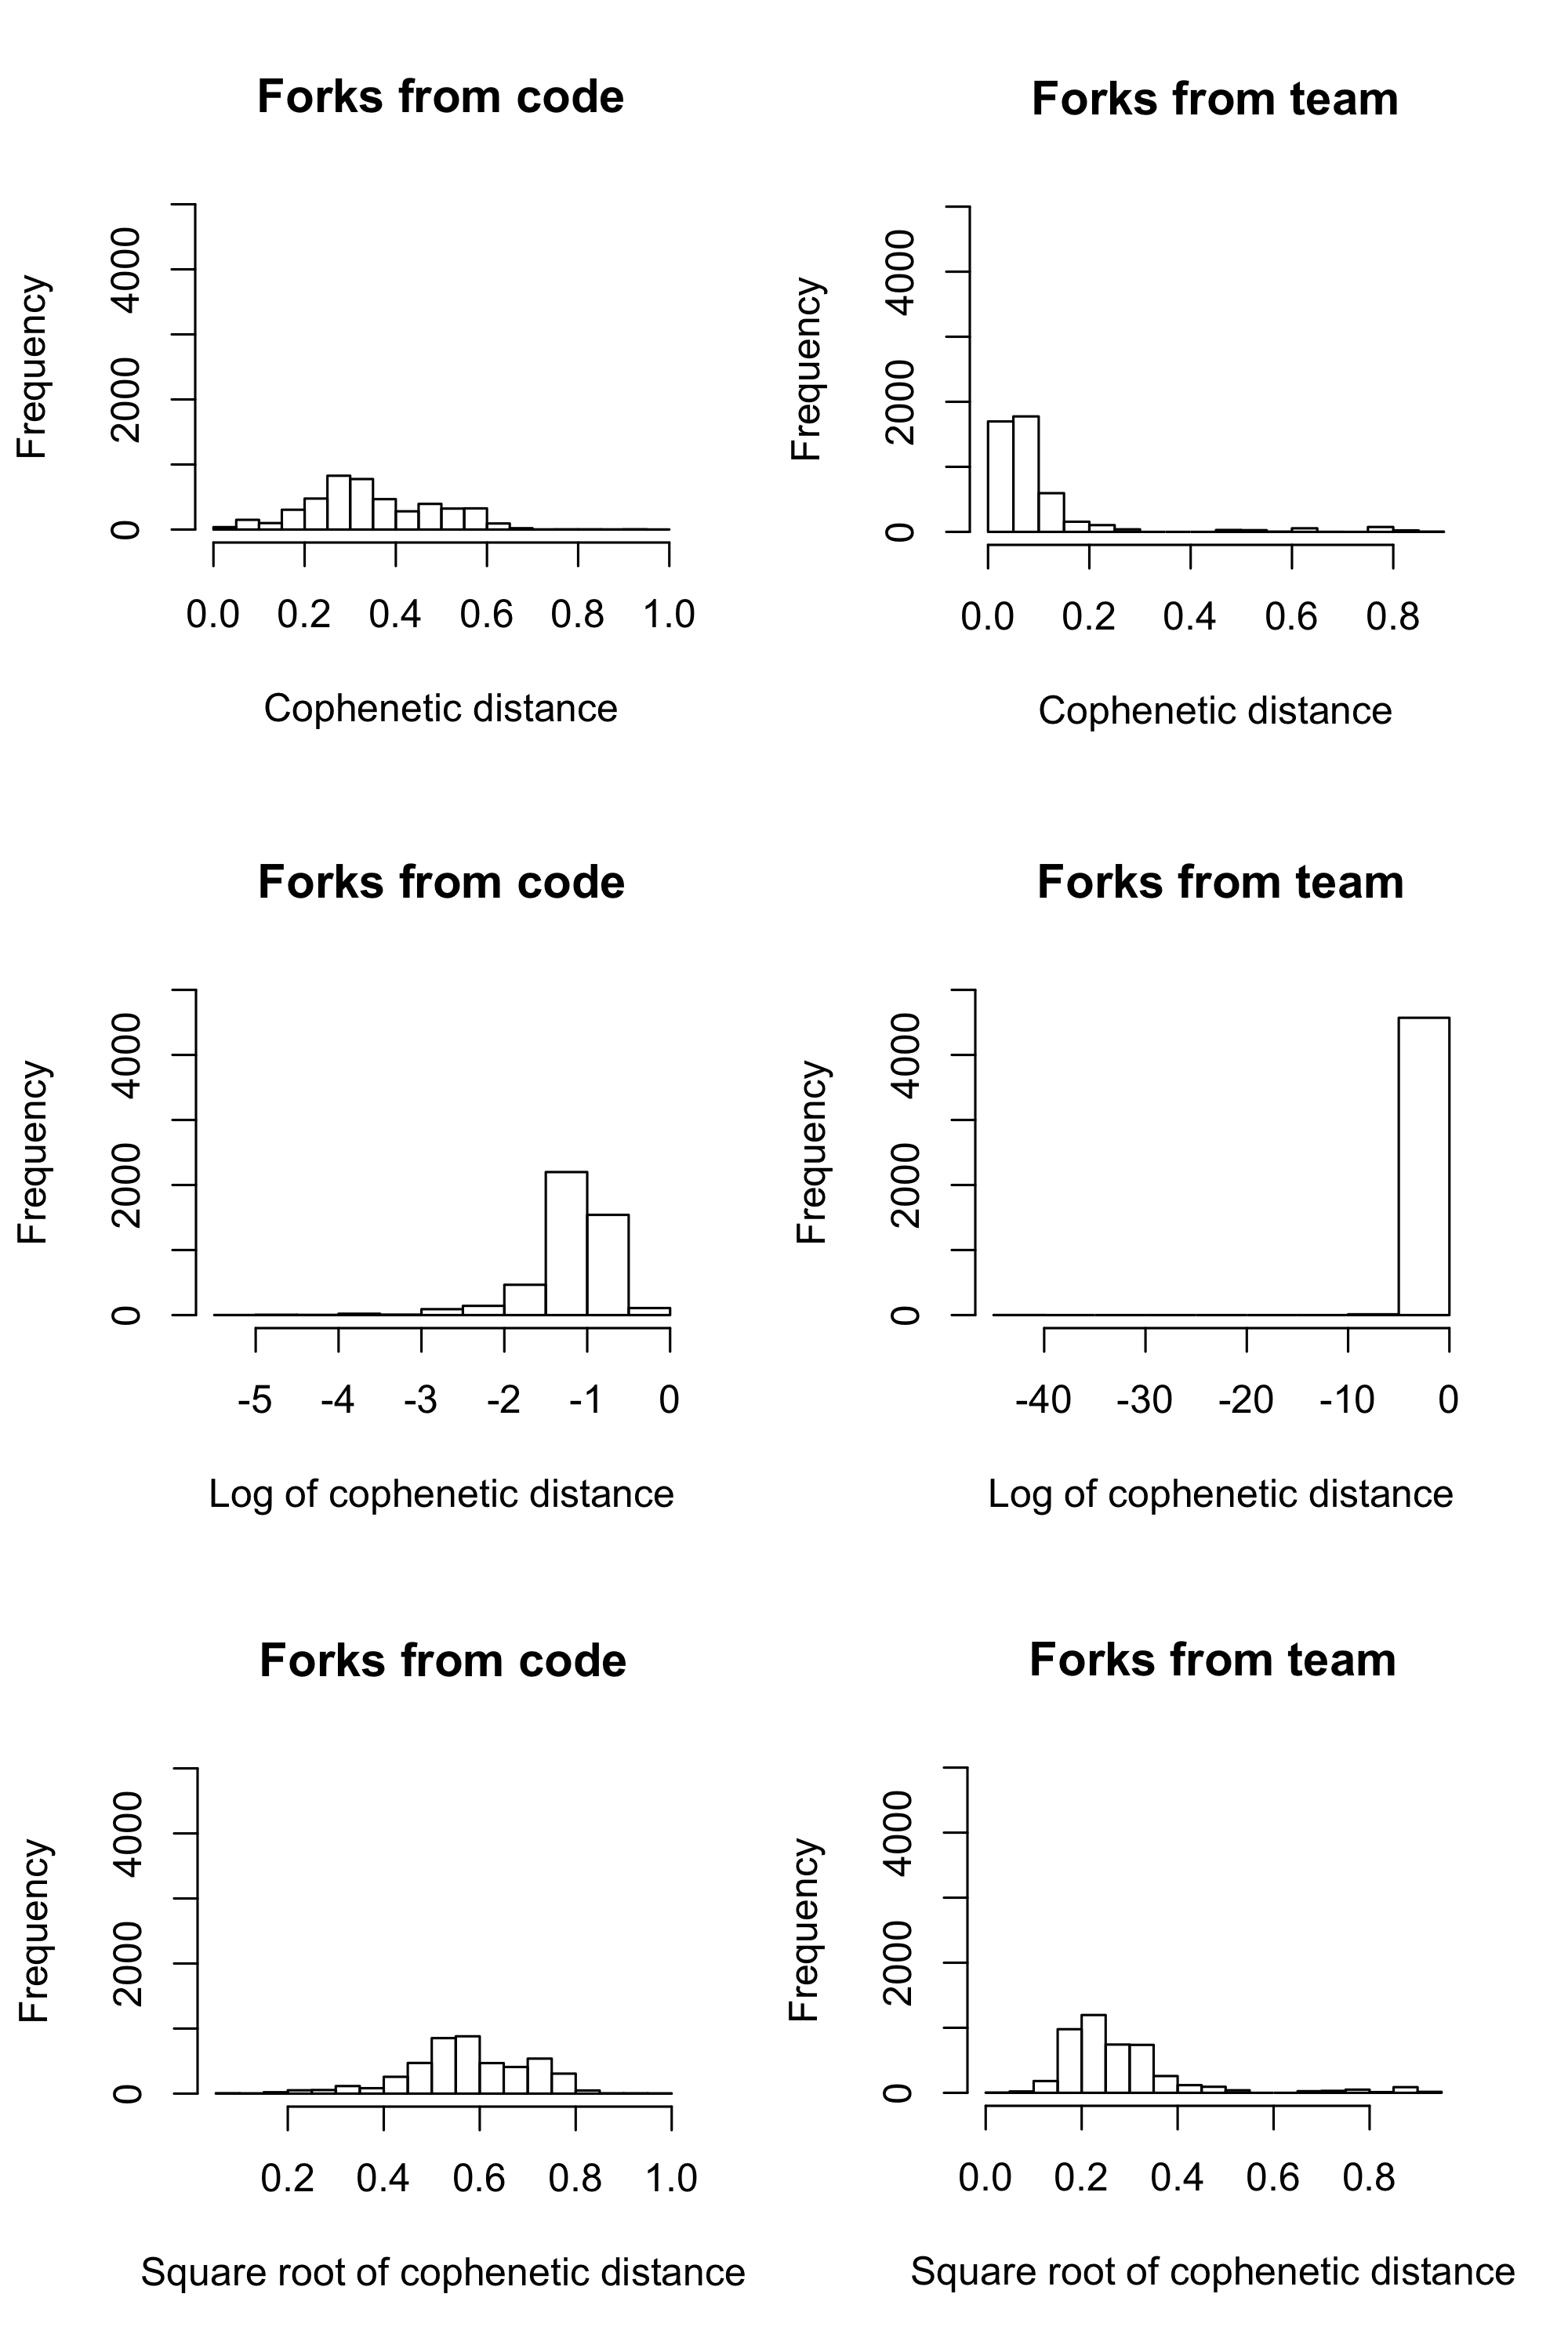
\includegraphics[width=\textwidth]{rq2_distributions.png}
  \caption{Histograms illustrating the distribution of the cophenetic distances: top row untransformed distances, middle row base-10 logarithm of the distances and bottom row square root of the distances.}
  \label{fig:rq2_distributions}
\end{figure}

\definition{Assumption 3: Homoscedasticity}{Two-way ANOVA assumes that the standard deviation of the data is the same for the data sets considered; performing a two-way ANOVA on heteroscedastic data sets increases the chance of false positives \citep[p.176]{McDonald2014b}.}

\noindent
Table \ref{table:ch4_rq2_sd} shows that the square root transformed data set is homoscedastic within reason, i.e. the ratio between the standard deviation of fork distances from team and code data is relatively small (0.1435011 / 0.1258846 = 1.1399417). Therefore, performing a two-way ANOVA on the square root transformed data should minimize the chance of false positives.

%-- table ----------
\begin{table}[H]
\caption{.}
\label{table:ch4_rq2_sd} 
\centering
\begin{tabu} to \linewidth{llr}
  \toprule
  Transformation applied & Data set & Standard deviation \\
  \midrule
  \multirow{2}{*}{Square root} \\
  & code & 0.1258846 \\
  & team & 0.1435011 \\
  \bottomrule
\end{tabu}
\end{table}


\subsubsection{Two-way analysis of variance}
The analysis involves the following steps:

\begin{enumerate}
\item{Distance matrices were computed from the data acquired for each fork, using the Gower technique, as the data is of various types (Boolean, integer, categorical, see table 3.1). Data obtained from code and team measurements was treated separately.}
\item{Trees were estimated from these distance matrices by applying the Neighbour-Joining (NJ) method, which was found to represent the distance matrix in an accurate way (as discussed under “checking assumptions for RQ2”).}
\item{A cophenetic distance matrix was obtained for the “code” and “team” data sets (the first nominal variable) for each project outcome, i.e. “collaboration”, “competition” and “discontinued fork” (the second nominal variable).}
\item{The pairwise distances between releases on the same branch were discarded, leaving a matrix of pairwise distances between forks.}
\item{Two-way ANOVA was performed on the square-root of the cophenetic distances (the measurement variable), as the square root transformed data is closer to a normal distribution than the raw data and is reasonably homoscedastic (as discussed under “checking assumptions for RQ2”).}
\end{enumerate}

The analysis of the square root transformed data with two-way ANOVA (table \ref{table:ch4_rq2_anova}) showed that the nominal variable “dataset” (i.e. “code” or “team”) has significant influence on the cophenetic distance between releases (p < 2e-16), but the nominal variable “outcome” (i.e. “cooperation”, “competition” or “discontinued branch”) does not (p = 0.7808). Therefore, the null hypothesis cannot be rejected.

%-- table ----------
\begin{table}[H]
\caption{Two-way ANOVA.}
\label{table:ch4_rq2_anova} 
\centering
\begin{tabu} to \linewidth{P{3.5cm}P{1.5cm}rrrP{1.5cm}}
  \toprule
  Nominal variable & Degrees of freedom & Sum squares & Mean squares & F value & Pr(>F) \\
  \midrule
  Data set ("team" or "code") & 1 & 194.632 & 194.632 & 10680.7077 & < 2e-16 \\
  \midrule
  Outcome (“competition”,
  “collaboration”
  or
  “discontinuation of a branch”) & 2 & 0.009 & 0.005 & 0.2475 & 0.7808 \\
  \bottomrule
\end{tabu}
\end{table}


% ----------------------------------------------------------------------------------------

\section{Interpretation in relation to the objectives}
This research set itself five objectives: review the current state of research, select suitable repositories to collect data, implement the analytical methods, analyse the data using methods from evolutionary biology, report for an audience of practitioners.

\subsection{Objective 1: Review the current state of research}
The first objective, to review the current state of research, showed that many similarities exist between biological and software evolution: biological concepts such as “ecosystem”, “lineage” and “evolution” have been used effectively to describe biological and software systems. There are however significant gaps, e.g. what constitutes a “gene” in a software context remains unclear. Furthermore, the literature research emphasizes that the study of forking is a lively research area.

However, to the best of my knowledge, there is very little work on transferring methods from evolutionary biology, in particular phylogenetic methods, to computer science. Therefore, primary research was required to assess whether the chosen methods are applicable to the study of software evolution in general and forking in particular.

\subsection{Objective 2:  Select suitable repositories to collect data}
The second objective, to select suitable repositories to collect data, showed that many open source repositories are accessible and can be mined for data on their release history and team composition. The source code had to be available online and additionally, the project's history back to the moment in time when the fork took place had to be available as well. Suitable projects were found and three were selected for analysis. The quantity of data collected justified the use of a database to store the data.

\subsection{Objective 3: Implement the analytical methods}
The third objective, to implement the analytical methods, was facilitated by the many libraries available for biological statistics. The methods and framework chosen are well documented, notably by \citet{Paradis2011} and software was implemented to apply these methods to the data. As the amount of data was large (table 4.5) and the methods were computationally intensive, the amount of time required for computation was larger than had been anticipated. Practitioners might be advised to plan for a long computation time. The software implemented for the research is documented in appendix 2.

\subsection{Objective 4: Analyse the data using methods from evolutionary biology}
The fourth objective, to analyse the data using methods from evolutionary biology, was addressed by answering two research questions (paragraph 2.1):
\definition{RQ1}{Can a threshold be determined beyond which two diverging development branches will be more likely to fork than to merge?}

The analysis of variance performed to answer RQ1 shows that the mean cophenetic distances from branches and forks are significantly heterogeneous for the projects studied. However, the research question sought a threshold that would permit to differentiate between branches and forks for any project. The plot in figure 4.4 was obtained by estimating the phylogenetic tree of each project separately, applying the Neighbour-Joining (NJ) method and subsequently by calculating the cophenetic distances between releases inside each project (“Branches”) and between releases on different forks (“Forks”), ordered by mean cophenetic distance. The plot shows that within each forked project, the distance between releases on the same branch is always smaller than the distance between releases on different forks. However, this does not hold for releases on any project, as the distance between branches of Apache OpenOffice (AOO) is larger than the distance between releases on the Linux / Android forks.

\begin{figure}[H]
  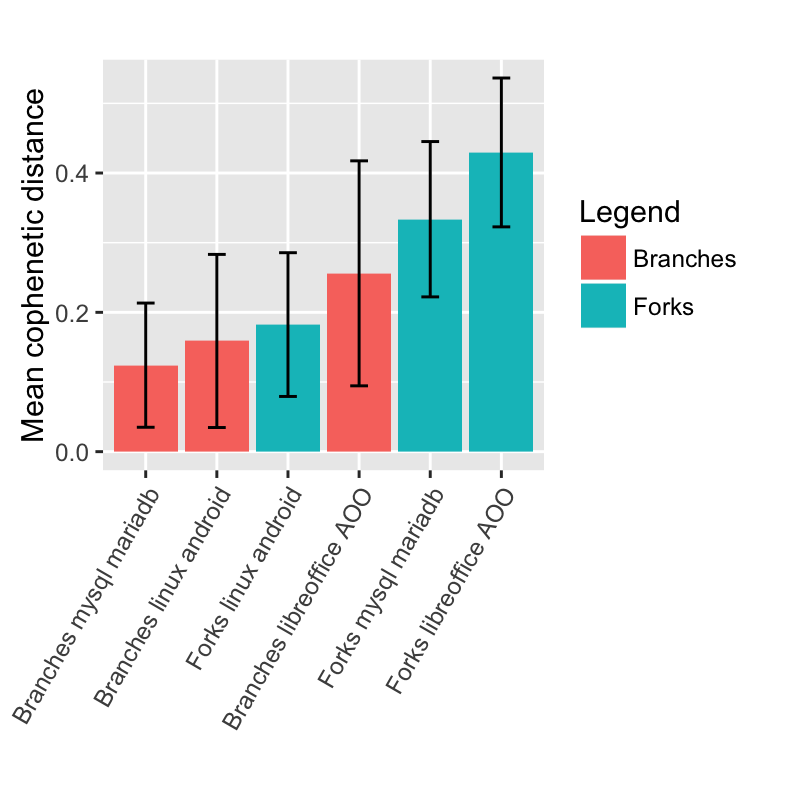
\includegraphics[width=\textwidth]{RQ1.png}
  \caption{Plot of the mean cophenetic distances between releases and their standard deviation for each fork case separately, sorted by distance.}
  \label{fig:rq1}
\end{figure}


Therefore, based on the three cases analysed, no generally applicable threshold value could be determined. Nevertheless, within a given forked project, the mean dissimilarity between releases on different forks is always larger than the mean dissimilarity between releases on the same branch. It can therefore be assumed that potential forks could be detected using this method.

\definition{RQ2}{Can the likely outcome (cooperation, competition or discontinuation) of an ongoing fork be predicted?}

The results for RQ2 are negative: the null hypothesis that forks with different outcomes are indistinguishable based on code and organizational measurements cannot be rejected. Consequently, no evidence could be found that the outcome of a project (i.e. “cooperation”, “competition” or “discontinued branch”) correlates with the distance between forks. Therefore, measurements of code and team characteristics are not sufficient to predict the outcome of a fork.

\subsection{Objective 5: Report}
The fifth objective was to report on the research for an audience of practitioners. Recommendations for practitioners are included in paragraph 4.4.

%----------------------------------------------------------------------------------------

\section{Interpretation in relation to the research aim}
The aim of the research was to assess whether methods and techniques from phylogenetics can be of real-world usefulness for the management of forks of open source software projects. 

\subsection{Forks as risks}
Research question 1 (RQ1) dealt with forks as a risk. If forks are a risk, then detecting development strands that are about to fork, before the actual fork happens, can be helpful to prevent the fork. The result for RQ1 provide evidence that, based on the three examples of forked projects examined, it is possible to detect a potential fork by examining the cophenetic distance matrix of the releases within a project. However, no generally applicable threshold could be determined beyond which any project would be likely to fork. Therefore phylogenetic methods are useful to detect potential forks, although to a lesser extent than expected.

\subsection{Forks as opportunities}
Research question 2 (RQ2) dealt with forks as opportunities. If the outcome of a fork can be predicted, then a purposeful fork could be used to solve technical, political or license problems. The result for RQ2 did not provide evidence that the outcome of a fork can be predicted solely based on measurements of code churn, team composition, edit frequency and code ownership. Therefore phylogenetic methods based on these measurements are not sufficient to predict the outcome of a fork.

\subsection{Tree thinking}
Phylogenetic trees are a depiction of estimated evolutionary relationships and could potentially be used to depict the state of a forked software project. This is illustrated in figure \ref{fig:example_tree1}, showing an example phylogenetic tree, constructed by subsampling the data collected for the MySQL / MariaDB fork. 

\citet{Baum2008b} coined the term “tree-thinking” to sum up the skills required to interpret phylogenetic trees. Basic concepts of “tree-thinking” could be ported to computer science and help to communicate about software evolution in general and forking processes in particular. \citet{Baum2008b} list terms useful for conceptualizing the evolutionary relationships captured in phylogenetic trees:

\begin{description}
\dt{Relatedness}{According to \citet{Baum2008b}, the term “relatedness” is used in biology to describe the recency of common ancestry. Ported to software evolution, relatedness could refer to the number of software releases between a pair of releases and their last common ancestor. For example, in figure \ref{fig:example_tree1}, MariaDB 10.0.1 and MySQL 5.6.5 (highlighted in blue) are more related to each other through their common ancestor MySQL 5.0.0 (highlighted in green), than to the majority of releases within their respective projects.}

\dt{Clade}{In biological evolution, a clade is a group comprised of an ancestor and all its descendants \citep{Baum2008b}. In the study of software evolution, a clade could be defined as the release which introduced a feature and all subsequent releases. For example, in the MySQL/MariaDB fork depicted in figure \ref{fig:example_tree1}, the MySQL 5.6.11, MySQL 5.7 and MySQL 8 series branched at the same node (highlighted in purple), which suggests that they share one or more important features.}

\dt{Parsimony}{The principle of parsimony states that the most likely tree is the one which displays the data in the simplest way, i.e. the tree that implies the least number of evolutionary changes \citep{Baum2008b}. While this might not be what actually happened, the parsimony principle allows reducing complex relationships to a manageable size. Therefore, parsimony could be applied to depict and grasp the release history of complex software projects.  For example, in figure \ref{fig:example_tree1}, MySQL 8.0.0 (highlighted in yellow) is depicted as closely related to the MySQL 5.7 series.}

\dt{Convergent evolution}{Similarities between biological organisms can arise in unrelated clades as a result of convergent evolution \citep{Baum2008b}. In computer science, convergent evolution could be used to describe the situation that arises when unrelated software develops similar features. For example, several mobile operating systems have opted to distribute their software through an online "application store"; however, this does not imply that their source code stems from a common origin: as discussed in paragraph 4.1, the Android operating system is related to the Linux operating system; there are however other mobile operating systems (e.g. iOS) which are unrelated to Linux, but have opted for a similar "application store" distribution model.}
\end{description}

\begin{figure}[H]
  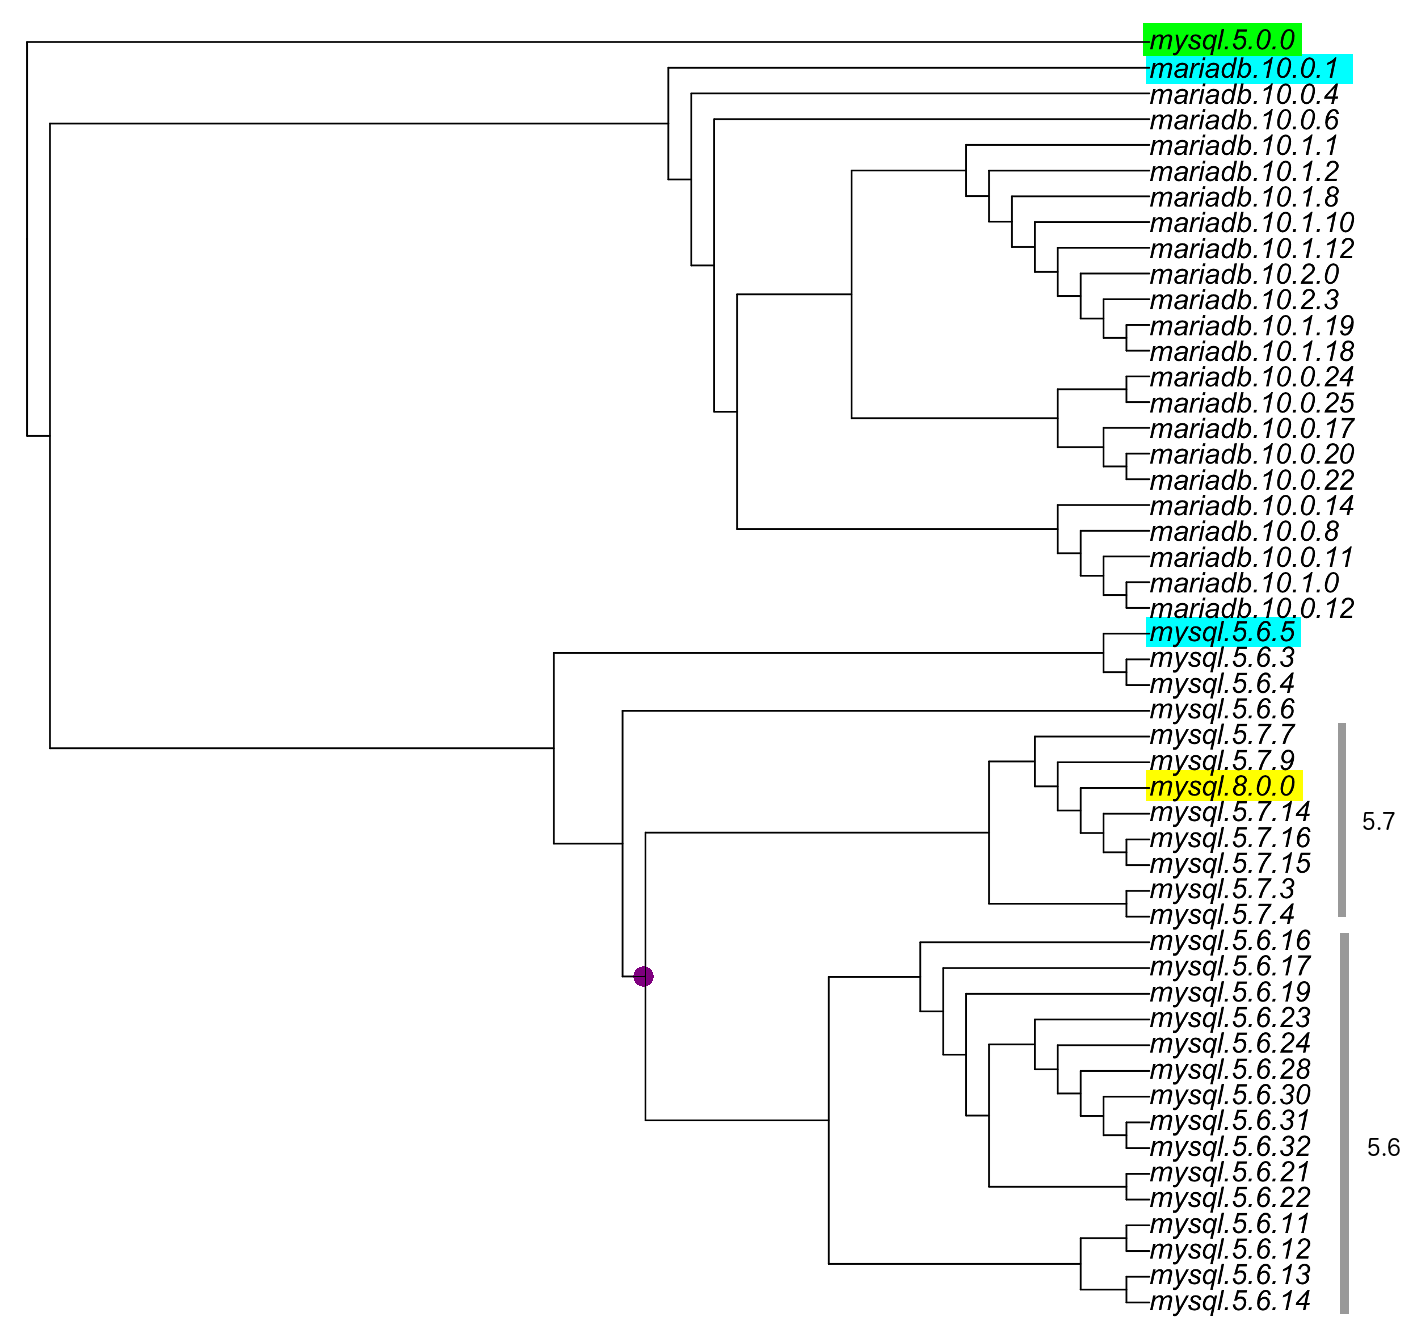
\includegraphics[width=\textwidth]{example_tree1.png}
  \caption{An example tree of the MySQL / MariaDB fork, obtained by subsampling fifty branches and ten thousand measurements.}
  \label{fig:example_tree1}
\end{figure}

%----------------------------------------------------------------------------------------

\section{Summary of Chapter 4}
Three forked open source projects were selected for carrying out case studies of forks with different reasons and outcomes. The three forks selected were: (1) MySQL server / MariaDB server, a database engine that forked due to licensing and community issues, (2) Linux kernel / Android kernel, a “friendly” fork, due to diverging commercial and technical strategies, and (3) Apache OpenOffice / LibreOffice, a fork due to the abandonment of the original project. 

Data was acquired from the online repositories of each project. Data was exported in a format suitable for analysis, re-encoded and cleaned-up where necessary. The previously discussed methods for estimating phylogenetic trees were implemented using the R language for statistical computing. It was determined that an analysis of the variance of the mean distances between branches and forks was a suitable statistical technique for answering the first research question (RQ1). The assumptions upon which this technique is predicated were checked. It was found that the Neighbour-Joining technique applied to the square root of the data was most likely to avoid false positives. Thereafter, it was determined that an analysis of the variance of the mean distances between forks with different outcomes, based on two data sets obtained from code-base and organizational measurements was a suitable statistical method for answering the second research question (RQ2). It was found that similar techniques as for RQ1 had to be applied to avoid false positives for RQ2. 

Interpretation yielded that branches can be told from forks within a project using methods for estimating phylogenetic trees, but no generally applicable threshold value between branches and forks could be determined. Therefore, the likelihood that a project will fork cannot be assessed with certainty. Nevertheless, branches that have wandered far away from the main development effort can be detected. No correlation could be found between the topology of the tree and the outcome of a fork, therefore the likely outcome of a fork cannot be foretold using these methods and measurements. An attempt was made at porting several concepts borrowed from biological evolution to describe relationships in software evolution.
